% 04_body.tex — Materiales y métodos, Resultados, Discusión, Conclusiones (IMRAD)
% ════════════════════════════════════════════════════════════════════════════
% Cadena aritmética del pipeline (verificada con logs 2026-09-16/18/20):
%   541 (Scopus 312 + WoS 188 + IEEE 41)  [+ SciELO/LILACS: ver 00_datos_pendientes]
%   − 188 duplicados                   = 353 únicos
%   −  48 tipo −  66 año               = 239 prefiltrados (2015-2026)
%   −   9 sin cuartil SCImago 2024     = 230 (Q1 130 + Q2 61 + Q3 21 + Q4 18)
%   Doble cribado humano → 2 incluidos (Palacio-Morales 2021; Murugesan 2020)
% Tablas del cuerpo (máx. 8): busqueda, confusion_inter, studies, comunidades,
%   auditoria, mapeo_rqs, transferibilidad  (= 7).
% Figuras del cuerpo (máx. 8): causal, quartil, prisma, mapa_evidencia,
%   produccion, vos, hoja_ruta (= 7).
% ════════════════════════════════════════════════════════════════════════════
\emergencystretch=1em

% ─────────────────────────────────────────────────────────────────────────────
\section{Materiales y métodos}
\label{sec:metodos}
% ─────────────────────────────────────────────────────────────────────────────

\subsection{Diseño del estudio, protocolo y guía de reporte}
\label{sub:diseno}

Se realizó una \textbf{revisión de alcance} con un componente bibliométrico
explícito, siguiendo el marco de Arksey y O'Malley
\parencite{arksey2005scoping} con las mejoras de Levac et~al.\
\parencite{levac2010scoping}, las precisiones de Munn et~al.\
\parencite{munn2018scoping} y la guía del \textit{Joanna Briggs Institute}
\parencite{peters2020scoping}. Se reportó conforme a PRISMA-ScR
\parencite{tricco2018prismascr} (lista de verificación en el
Apéndice~\ref{apx:prisma}); el diagrama de flujo sigue la convención de
PRISMA~2020 \parencite{page2021prisma}. El protocolo se depositó en OSF
(\OSFTexto) antes de ejecutar la búsqueda.

\paragraph{Desviaciones respecto del protocolo.} Dos criterios de
elegibilidad se modificaron después del registro y antes del cribado
sobre el corpus definitivo: (i)~el umbral de cuartil SJR se amplió de
Q1--Q2 a Q1--Q4 el 13 de agosto de 2026, al comprobar que la búsqueda no
había restringido por cuartil y que, en un dominio de nicho, un umbral
alto podía descartar evidencia \textit{in-domain}; y (ii)~la ventana
temporal se extendió hasta 2026 para incorporar publicaciones
\textit{early access}. La primera enmienda fue posterior a un cribado
preliminar sobre Q1--Q2 que había identificado un único estudio, es
decir, se tomó con conocimiento parcial de los resultados; se declara
como fuente potencial de sesgo y se acota con el análisis de
sensibilidad de \ref{sub:sensibilidad}.

\paragraph{Justificación del diseño.} Se descartó una revisión narrativa
y una revisión sistemática agnóstica del dominio por tres razones.
Primero, la pregunta es de mapeo (extensión, naturaleza y madurez de la
evidencia), no de efectividad, por lo que no procede un metaanálisis.
Segundo, el tamaño reducido del corpus es un resultado a sostener, y solo
una estrategia de búsqueda reproducible con un embudo de decisiones
auditable distingue ``no hay evidencia'' de ``no se buscó
exhaustivamente'' \parencite{lang2007empty,yaffe2012empty}; la
literatura transferible de otros dominios se sintetiza de forma
narrativa en \ref{sub:transferibilidad}, de modo que el diseño combina
ambos enfoques. Tercero, el componente bibliométrico caracteriza el campo
adyacente para interpretar el vacío. Una revisión agnóstica (control de
pH con AA en cualquier industria) habría respondido otra pregunta y
solaparía revisiones existentes sobre bioprocesos y efluentes.

\subsection{Criterios de elegibilidad}
\label{sub:criterios}

Los criterios se definieron bajo el marco PICOC descrito en
\ref{sub:rqs}.

\noindent\textbf{Inclusión.}
(a)~Artículos de revista originales publicados entre 2015 y 2026,
incluyendo registros \textit{early access} con año editorial 2026;
(b)~revista indexada en SJR (SCImago, edición 2024, criterio
\textit{best quartile}) con cuartil Q1--Q4;
(c)~aplicación de al menos una técnica de AA, de control avanzado o de
sensor virtual al pH del proceso de clarificación o encalado del jugo de
caña o remolacha; se consideró \emph{control avanzado} todo esquema
distinto de un PID de ganancia fija (MPC/NMPC, control difuso o
neuro-difuso, adaptativo) y se admitió la identificación o sintonía de
controladores mediante metaheurísticas o AA; y
(d)~reporte de al menos una métrica cuantitativa de desempeño.

\noindent\textbf{Exclusión.}
(a)~Actas de congreso, capítulos y series de libros;
(b)~fuera del rango temporal;
(c)~revista sin cuartil SJR en SCImago~2024;
(d)~procesos ajenos al lazo de pH de la clarificación azucarera
(fermentación alcohólica, tratamiento de aguas residuales, jugos de fruta,
farmacéutica, extracción mineral, análisis sensorial); y
(e)~pH tratado solo como descriptor químico o variable de entrada, sin
objetivo de predicción, estimación o control.

\noindent\textbf{Justificación y riesgos de los criterios formales.}
Restringir a artículos de revista con cuartil SJR persigue una calidad
editorial verificable y homogénea; el rango completo Q1--Q4 evita
sesgar \textit{a priori} un dominio de nicho hacia los cuartiles
superiores. Sin embargo, estos criterios tienen un costo: excluyen la
literatura de ingeniería publicada en actas y las revistas no indexadas
en SCImago, que en control de procesos pueden concentrar parte de la
evidencia. Por esa razón se pre-especificó una caracterización de los
registros \textit{in-domain} excluidos por estos criterios
(\ref{sub:sensibilidad}); los resultados se reportan por separado de los
estudios que cumplen todos los criterios.

\noindent\textbf{Ventana temporal.} La ventana 2015--2026 abarca la
difusión del aprendizaje profundo y del aprendizaje por refuerzo profundo
en ingeniería \parencite{krizhevsky2012imagenet,mnih2015human} y la
literatura reciente sobre NMPC con identificación no lineal. Un
\textit{cutoff} anterior habría incorporado trabajos fundacionales que,
siendo relevantes como contexto (\ref{sub:otros_dominios}), no reflejan
el estado actual del campo.

\subsection{Fuentes de información y estrategia de búsqueda}
\label{sub:fuentes}

Se consultaron \textbf{cinco bases de datos} el \FechaBusqueda:
Scopus, Web of Science e IEEE~Xplore, más \textbf{SciELO} y \textbf{LILACS}
para incrementar la cobertura de literatura latinoamericana y brasileña en
español y portugués, dada la relevancia del sector azucarero en Brasil.
Se ejecutaron nueve consultas booleanas (tres por base original, mapeadas
1~a~1 con las tres preguntas de investigación) y una consulta combinada
adicional por base para SciELO y LILACS, adaptada a su sintaxis
(Tabla~\ref{tab:busqueda}; cadenas completas en el
Apéndice~\ref{apx:queries_multibase}). Las consultas incorporaron cláusulas
\texttt{AND~NOT} para excluir dominios tópicamente ruidosos detectados en
una búsqueda piloto (\textit{wastewater}, \textit{bioethanol},
\textit{fermentation broth}, \textit{pharmaceutical}, \textit{soil},
\textit{blood}, \textit{wine}, \textit{dairy}, \textit{bioreactor}).

El uso de \texttt{AND~NOT} introduce un riesgo de sesgo de selección: un
término de exclusión amplio puede eliminar registros \textit{in-domain}
que mencionen tangencialmente, por ejemplo, \textit{wastewater} o
\textit{bioreactor}. Se mitigó calibrando cada término de exclusión en la
búsqueda piloto sobre registros ya identificados como ruido temático y no
sobre supuestos \textit{a~priori}. No se ejecutó, en cambio, una búsqueda
de control sin \texttt{AND~NOT} ni un rastreo sistemático de citas
(\textit{citation chasing}) sobre los estudios incluidos; por tanto, la
pérdida de algún registro marginal no puede descartarse y se declara como
limitación (\ref{sub:limitaciones}).

% Tabla de consultas booleanas (apaisada). Extraida de 04_body.tex
\newgeometry{margin=2cm}
\begin{landscape}
\sloppy
\hfuzz=500pt
\emergencystretch=3em
\begin{longtblr}[
caption={\textit{Consultas booleanas empleadas en la búsqueda sistemática
en Scopus, Web of Science e IEEE~Xplore. Correspondencia 1 a 1 con las
preguntas de investigación: $Q_1\!\rightarrow$\,RQ1 (modelado/sensores
virtuales); $Q_2\!\rightarrow$\,RQ2 (control avanzado vs.\ PID);
$Q_3\!\rightarrow$\,RQ3 (ML/RL/híbridos y barreras). Se muestra el formato
Scopus TITLE-ABS-KEY; los equivalentes semánticos por base, incluidas las
cadenas específicas para SciELO y LILACS, se documentan en el
Apéndice~\ref{apx:queries_multibase}.}},
label={tab:busqueda},
]{colspec={X[1.2,c]X[3.4,l]X[14.5,l]X[0.9,c]},width=\linewidth,
  rowsep=3pt,
  hline{1,2,Z}={0.6pt},row{1}={font=\bfseries}}
$Q_i$ & Foco temático (RQ) &
Cadena booleana (Scopus TITLE-ABS-KEY) & $N$ \\
$Q_1$ & Modelado y sensores virtuales de pH (RQ1) &
{\raggedright\scriptsize\ttfamily TITLE-ABS-KEY(("pH control" OR "pH monitoring" OR
"pH prediction" OR "pH regulation" OR "pH measurement" OR "acidity control"
OR "alkalinity control" OR "juice acidity" OR "lime dosage" OR
"calcium hydroxide" OR "milk of lime") AND ("sugar mill" OR "sugarcane" OR
"cane juice" OR "sugar juice" OR "sugar industry" OR "juice clarification"
OR "liming process" OR "defecation" OR "sulfitation" OR "sugar beet" OR
"sugar factory" OR "saccharum") AND ("soft sensor" OR "virtual sensor" OR
"inferential sensor" OR "identification" OR "data-driven model" OR
"neural network" OR "LSTM" OR "predictive model" OR "regression model"))
AND NOT TITLE-ABS-KEY("wastewater" OR "soil pH" OR "fermentation broth" OR
"bioethanol" OR "pharmaceutical" OR "bioreactor" OR "wine" OR "beer" OR
"dairy")}
& 18 \\
$Q_2$ & Control avanzado (MPC/NMPC, difuso, metaheurísticas) vs.\ PID (RQ2) &
{\raggedright\scriptsize\ttfamily TITLE-ABS-KEY(("model predictive control" OR "NMPC"
OR "nonlinear MPC" OR "fuzzy logic" OR "takagi-sugeno" OR "neuro-fuzzy"
OR "adaptive control" OR "intelligent control" OR "PID tuning" OR
"optimal control" OR "pattern search" OR "particle swarm" OR
"genetic algorithm" OR "differential evolution" OR "bayesian optimization")
AND "pH" AND ("sugar mill" OR "sugarcane" OR "cane juice" OR "sugar juice"
OR "juice clarification" OR "liming process" OR "defecation" OR
"sulfitation" OR "sugar industry" OR "sugar beet" OR "sugar factory"))
AND NOT TITLE-ABS-KEY("wastewater" OR "bioethanol" OR "fermentation broth"
OR "pharmaceutical" OR "soil" OR "blood" OR "wine" OR "dairy" OR
"desalination" OR "anaerobic digestion" OR "bioreactor")}
& 60 \\
$Q_3$ & ML/RL/híbridos y barreras de adopción (RQ3) &
{\raggedright\scriptsize\ttfamily TITLE-ABS-KEY(("machine learning" OR "deep learning"
OR "neural network" OR "artificial intelligence" OR "random forest" OR
"gradient boosting" OR "XGBoost" OR "lightGBM" OR "support vector" OR
"reinforcement learning" OR "deep reinforcement learning" OR "DDPG" OR
"PPO" OR "Q-learning" OR "hybrid model" OR "grey-box model" OR
"physics-informed" OR "digital twin" OR "transfer learning") AND "pH" AND
("sugar" OR "sugarcane" OR "cane juice" OR "sugar juice" OR
"clarification" OR "liming" OR "sugar mill" OR "sugar industry" OR
"sugar beet" OR "juice purification" OR "sugar factory" OR "defecation"))
AND NOT TITLE-ABS-KEY("wastewater" OR "bioethanol" OR "pharmaceutical" OR
"soil" OR "blood" OR "bioreactor" OR "desalination" OR "wine" OR "beer"
OR "fermentation broth")}
& 463 \\
\SetCell{c=3}\mbox{\textbf{Total bruto (nueve consultas, tres bases,
con duplicados intra e inter-fuente)}} & & & \textbf{541} \\
\SetCell{c=3}\mbox{\textbf{+ Adicionales SciELO y LILACS (ver Apéndice~\ref{apx:queries_multibase})}}
& & & \textbf{\NSciELOLILACS} \\
\end{longtblr}
\nolinenumbers
\begin{Nota}[Nota]{\linewidth}{Elaboración propia. Los valores de $N$
corresponden a las ejecuciones del \FechaBusqueda y fueron
verificados desde los archivos RIS exportados. Desglose por base original:
Scopus $=312$ ($Q_1{=}11$, $Q_2{=}32$, $Q_3{=}269$);
WoS $=188$ ($Q_1{=}3$, $Q_2{=}18$, $Q_3{=}167$);
IEEE~Xplore $=41$ ($Q_1{=}4$, $Q_2{=}10$, $Q_3{=}27$).
SciELO y LILACS se ejecutaron con consulta Q4 adaptada a DeCS/MeSH; los
recuentos exactos se reportan en la Tabla~\ref{tab:queries_multibase}
(Apéndice~\ref{apx:queries_multibase}). Sintaxis WoS: sustituir
\texttt{TITLE-ABS-KEY} por \texttt{TS=} y \texttt{AND~NOT} por
\texttt{NOT~TS=}. Sintaxis IEEE~Xplore: operadores directos sobre
\textit{All~Metadata} sin prefijo de campo.}
\end{Nota}
\nolinenumbers
\end{landscape}
\restoregeometry

\linenumbers

\subsection{Proceso de selección}
\label{sub:seleccion}

Sobre el corpus bruto se aplicaron seis etapas secuenciales.

\paragraph{Etapa~1: Deduplicación.}
Emparejamiento difuso de títulos con \texttt{rapidfuzz} (umbral 95\,\%)
complementado por cruce por DOI: se eliminaron 188~duplicados (34.8\,\%),
quedando 353~registros únicos.

\paragraph{Etapa~2: Prefiltrado por tipo y año.}
Se retuvieron los artículos de revista (\texttt{TY=JOUR}), descartándose
actas, capítulos y series de libros ($n=48$), y se aplicó la ventana
2015--2026 ($n=66$), quedando 239~registros.

\paragraph{Etapa~3: Anotación y filtro por cuartil SJR.}
A los 239~registros se les asignó el cuartil SJR de su revista mediante
cruce jerárquico con SCImago~2024: primero por ISSN (49\,167~entradas) y,
en su defecto, por título normalizado (30\,992~entradas). Se
localizaron 232~revistas (97.1\,\%; ISSN: 213, título: 19). La
distribución fue Q1$=130$~(56.5\,\%), Q2$=61$~(26.5\,\%),
Q3$=21$~(9.1\,\%) y Q4$=18$~(7.8\,\%); 9~registros (3.8\,\%) carecían de
cuartil utilizable (7~revistas ausentes de SCImago~2024 y 2~con
correspondencia pero sin cuartil asignado) y se excluyeron, quedando
230~registros (Figura~\ref{fig:quartil}).

\nolinenumbers
\begin{figure}[H]
\centering
\captionsetup{width=0.9\textwidth}
\caption{Distribución de los 239~artículos de revista prefiltrados
(2015--2026) por cuartil SJR (SCImago 2024, \textit{best quartile});
los 230~registros Q1--Q4 se retuvieron y los 9~sin cuartil se excluyeron.}
\label{fig:quartil}
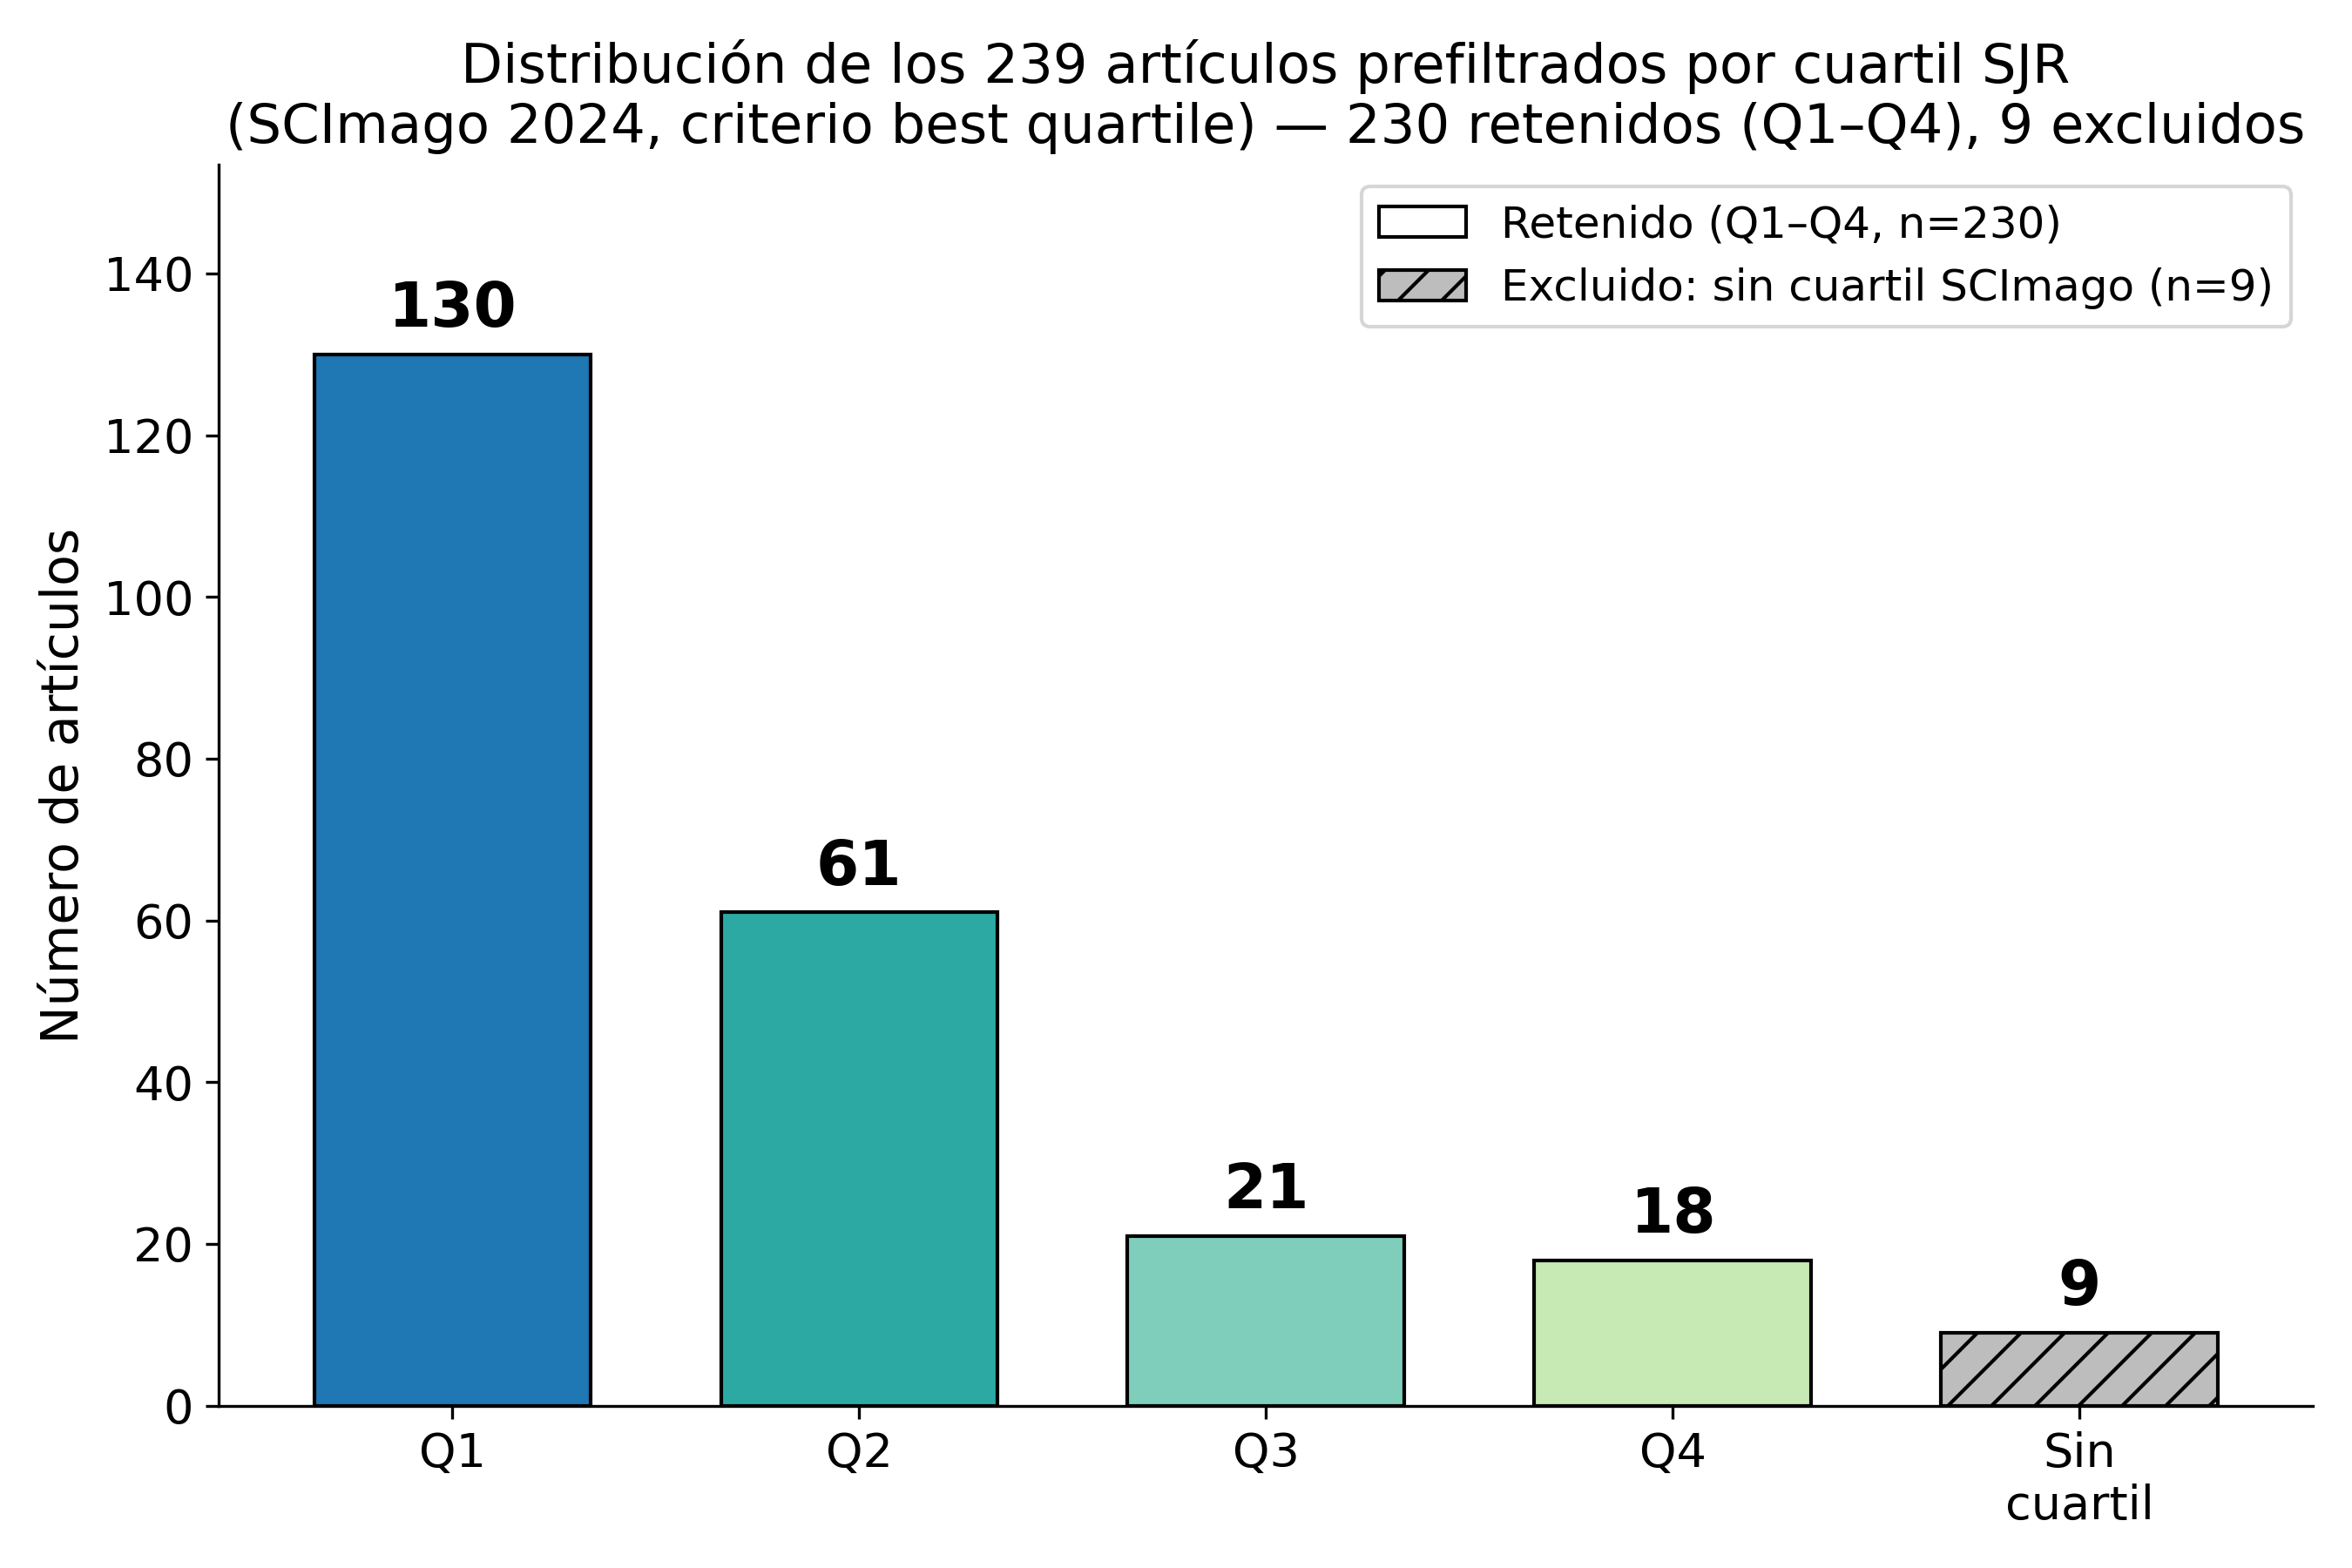
\includegraphics[width=0.85\textwidth,height=0.55\textheight,keepaspectratio]{Filtered_quartil.png}
\begin{Nota}[Nota]{0.9\textwidth}{Elaboración propia a partir del corpus
prefiltrado. La amplitud del umbral Q1--Q4 se justifica en
\ref{sub:criterios}.}
\end{Nota}
\end{figure}
\linenumbers

\paragraph{Etapa~4: Doble cribado humano independiente y ciego.}
\label{etapa:doble_cribado}
Los 230~registros fueron cribados por título y resumen por \textbf{dos
revisores humanos de forma independiente y ciega}. El \textbf{Revisor~1}
(autor principal) y el \textbf{Revisor~2} (\NombreCoRevisor) evaluaron
\textbf{el corpus completo} ($n=230$) con los criterios de
\ref{sub:criterios}. Ambos revisores operaron sin acceso a las
decisiones del otro ni a las del modelo de lenguaje. Las discrepancias
se resolverían por consenso y, de persistir, se remitirían a un tercer
revisor. La decisión consensuada es la \textbf{decisión primaria y
final}; su concordancia se reporta con $\kappa$ de Cohen inter-humano
(\ref{sub:fiabilidad_metodos}).

\paragraph{Etapa~5: Chequeo automático complementario (secundario).}
\label{etapa:llm_tertiary}
Como ejercicio de transparencia, y \emph{no} como sustituto del juicio
humano, el mismo corpus se procesó con un \textit{pipeline} automático de
dos niveles: (i)~un filtro léxico local en tres niveles (L0: términos de
exclusión de dominios ajenos; L1: presencia simultánea de vocabulario de
pH/encalado y de proceso azucarero; L2: vocabulario de AA o de
optimización), que resolvió 201~de 230~registros (87.4\,\%) como EXCLUIR
sin invocar al modelo; y (ii)~un modelo de lenguaje local (Llama~3~8B,
cuantización Q4\_0, vía Ollama; $T=0$) con un \textit{prompt} de seis
ejemplos sintéticos (Apéndice~\ref{apx:prompt}) sobre los 29~registros
restantes. Se fijó \textit{a~priori} un umbral de confianza de
derivación de $55\,\%$: un registro (una entrada de actas mal etiquetada
como artículo) cayó por debajo y se trató como EXCLUIR; de los 28
restantes, el modelo clasificó 2~como INCLUIR y 26~como EXCLUIR. El
\textit{prompt} de producción contenía, como ejemplo positivo, un
registro cuyo título, resumen y palabras clave reproducían los de uno de
los estudios incluidos; esta fuga de información se evaluó en
\ref{sub:sensibilidad}. Por ello, la concordancia modelo--humano se
reporta solo como métrica secundaria de reproducibilidad algorítmica.

\paragraph{Etapa~6: Lectura a texto completo y extracción.}
Los candidatos del doble cribado se leyeron a texto completo y los datos
se extrajeron de los PDF originales (no de los resúmenes). La verificación
confirmó \textbf{dos estudios incluidos}. La cadena acumulada es
$541 \rightarrow 353 \rightarrow 239 \rightarrow 230 \rightarrow 2$
(0.37\,\% del corpus bruto; 0.87\,\% del corpus Q1--Q4).

\subsection{Fiabilidad del cribado}
\label{sub:fiabilidad_metodos}

La fiabilidad se cuantificó en dos niveles. \emph{Primario}: concordancia
inter-humano entre los Revisores~1 y~2 sobre los 230~registros,
mediante el $\kappa$ de Cohen \parencite{mchugh2012interrater}, la
concordancia observada $P_0$, la sensibilidad, la precisión y $F_1$
tomando la decisión consensuada como referencia, con intervalos de Wilson
al 95\,\% \parencite{wilson1927probable}. Dado el desbalance esperado
entre clases, se reportó también el índice $\text{PABAK}=2P_0-1$
\parencite{byrt1993bias}, interpretado con la cautela descrita en la
literatura sobre la paradoja del $\kappa$ \parencite{feinstein1990high}.
\emph{Secundario}: la concordancia entre la decisión humana final y el
\textit{pipeline} automático (Apéndice~\ref{apx:kappa_notas}), etiquetada
como ejercicio de reproducibilidad algorítmica y no como validación del
cribado.

\subsection{Extracción de datos y evaluación del riesgo de sesgo}
\label{sub:extraccion}

Para los estudios incluidos se completó una matriz de extracción con
metadatos, técnica de modelado y control, variables manipuladas,
perturbaciones y controlada, origen de los datos, nivel de validación
(simulación, banco de pruebas, planta piloto, planta industrial) y
métricas reportadas. El nivel de madurez se expresó en la escala TRL de la
NASA \parencite{nasa2016trl}. Dado el corpus reducido se planificó una
síntesis narrativa \parencite{yaffe2012empty,lang2007empty}. El riesgo de
sesgo se evaluó con una herramienta \textit{ad~hoc} de cinco dominios
(Apéndice~\ref{apx:herramienta_sesgo}); su uso es opcional en
PRISMA-ScR y no pretende ponderar los resultados.

\subsection{Análisis bibliométrico y verificación léxica}
\label{sub:bibliometria}

Sobre el corpus Q1--Q4 ($n=230$) se construyó una red de co-ocurrencia de
palabras clave con \textit{bibliometrix} \parencite{ARIA2017959} y
\textit{VOSviewer} \parencite{vanecksoftware2010}; se retuvieron los
595~términos con frecuencia $\geq 2$ y los 120~nodos de mayor grado
ponderado. Las comunidades se detectaron con el algoritmo de Louvain
\parencite{blondel2008fast} y se reetiquetaron por su contenido
dominante. Como la ausencia de un término en una red con umbral de
frecuencia es evidencia indirecta, se añadió una \textbf{verificación
léxica independiente}: sobre los 353~registros únicos, sin filtrar por
tipo, año ni cuartil, se contó cuántos mencionan en título, resumen o
palabras clave cada concepto núcleo de las RQ, solo y en co-presencia con
vocabulario de pH/neutralización y de proceso azucarero (familias
de expresiones regulares en el Apéndice~\ref{apx:complementaria};
\textit{script} \texttt{12\_auditoria\_conceptual.py}).

\subsection{Análisis de sensibilidad}
\label{sub:sensibilidad}

Se realizaron tres análisis para acotar los sesgos de los criterios y del
chequeo automático.
(i)~\emph{Criterios de elegibilidad.} Entre los 353~registros únicos se
identificaron, mediante la verificación léxica, los que combinan pH y
proceso azucarero y no pasaron al cribado por tipo de documento o por
carecer de cuartil; se leyeron por título y resumen y se caracterizaron
descriptivamente (no constituyen un cribado formal ni entran en el
cálculo de $\kappa$).
(ii)~\emph{Filtro léxico local.} Los 201~registros resueltos por el
filtro L0--L2 se re-examinaron con un criterio más laxo, sin las reglas L0
ni el requisito de vocabulario de AA, y los que combinaban pH y proceso
azucarero se leyeron por título y resumen frente a los criterios.
(iii)~\emph{Fuga en el \textit{prompt}.} Los 29~registros que llegaron al
modelo se re-procesaron con el \textit{prompt} original y con uno
corregido (ejemplo positivo sintético de otra familia metodológica), con
el mismo modelo (resumen SHA-256
\texttt{365c0bd3c000\ldots}), $T=0$, y se compararon con la corrida de
producción.

% ─────────────────────────────────────────────────────────────────────────────
\section{Resultados}
\label{sec:resultados}
% ─────────────────────────────────────────────────────────────────────────────

\subsection{Búsqueda y selección de estudios}
\label{sub:res_prisma}

La búsqueda identificó $N=541$~registros en las tres bases originales
(Scopus $=312$; WoS $=188$; IEEE~Xplore $=41$); las búsquedas en SciELO y
LILACS no recuperaron ningún registro (\NSciELOLILACS{} resultados;
Tabla~\ref{tab:queries_multibase}), por lo que no modificaron el embudo.
Tras eliminar 188~duplicados quedaron 353~registros únicos; el prefiltrado
por tipo (48) y año (66) retuvo 239; y el filtro por cuartil, que excluyó
9~registros sin cuartil, dejó \textbf{230~artículos Q1--Q4}
(130~Q1, 61~Q2, 21~Q3 y 18~Q4). El cribado doble confirmó \textbf{dos
estudios incluidos}: \cite{palaciomorales2021optimiza}, en una revista
Q2, y \cite{murugesan2020computeraided}, en una revista Q3
(Figura~\ref{fig:prisma}).

\nolinenumbers
\begin{figure}[H]
\centering
\captionsetup{width=0.9\textwidth}
\caption{Diagrama de flujo PRISMA-ScR de la revisión de alcance.
Cadena verificada:
$N_{\text{bruto}}=541 \rightarrow n_{\text{únicos}}=353 \rightarrow
n_{\text{prefiltrado}}=239 \rightarrow n_{\text{Q1--Q4}}=230 \rightarrow
n_{\text{incluido}}=2$.}
\label{fig:prisma}
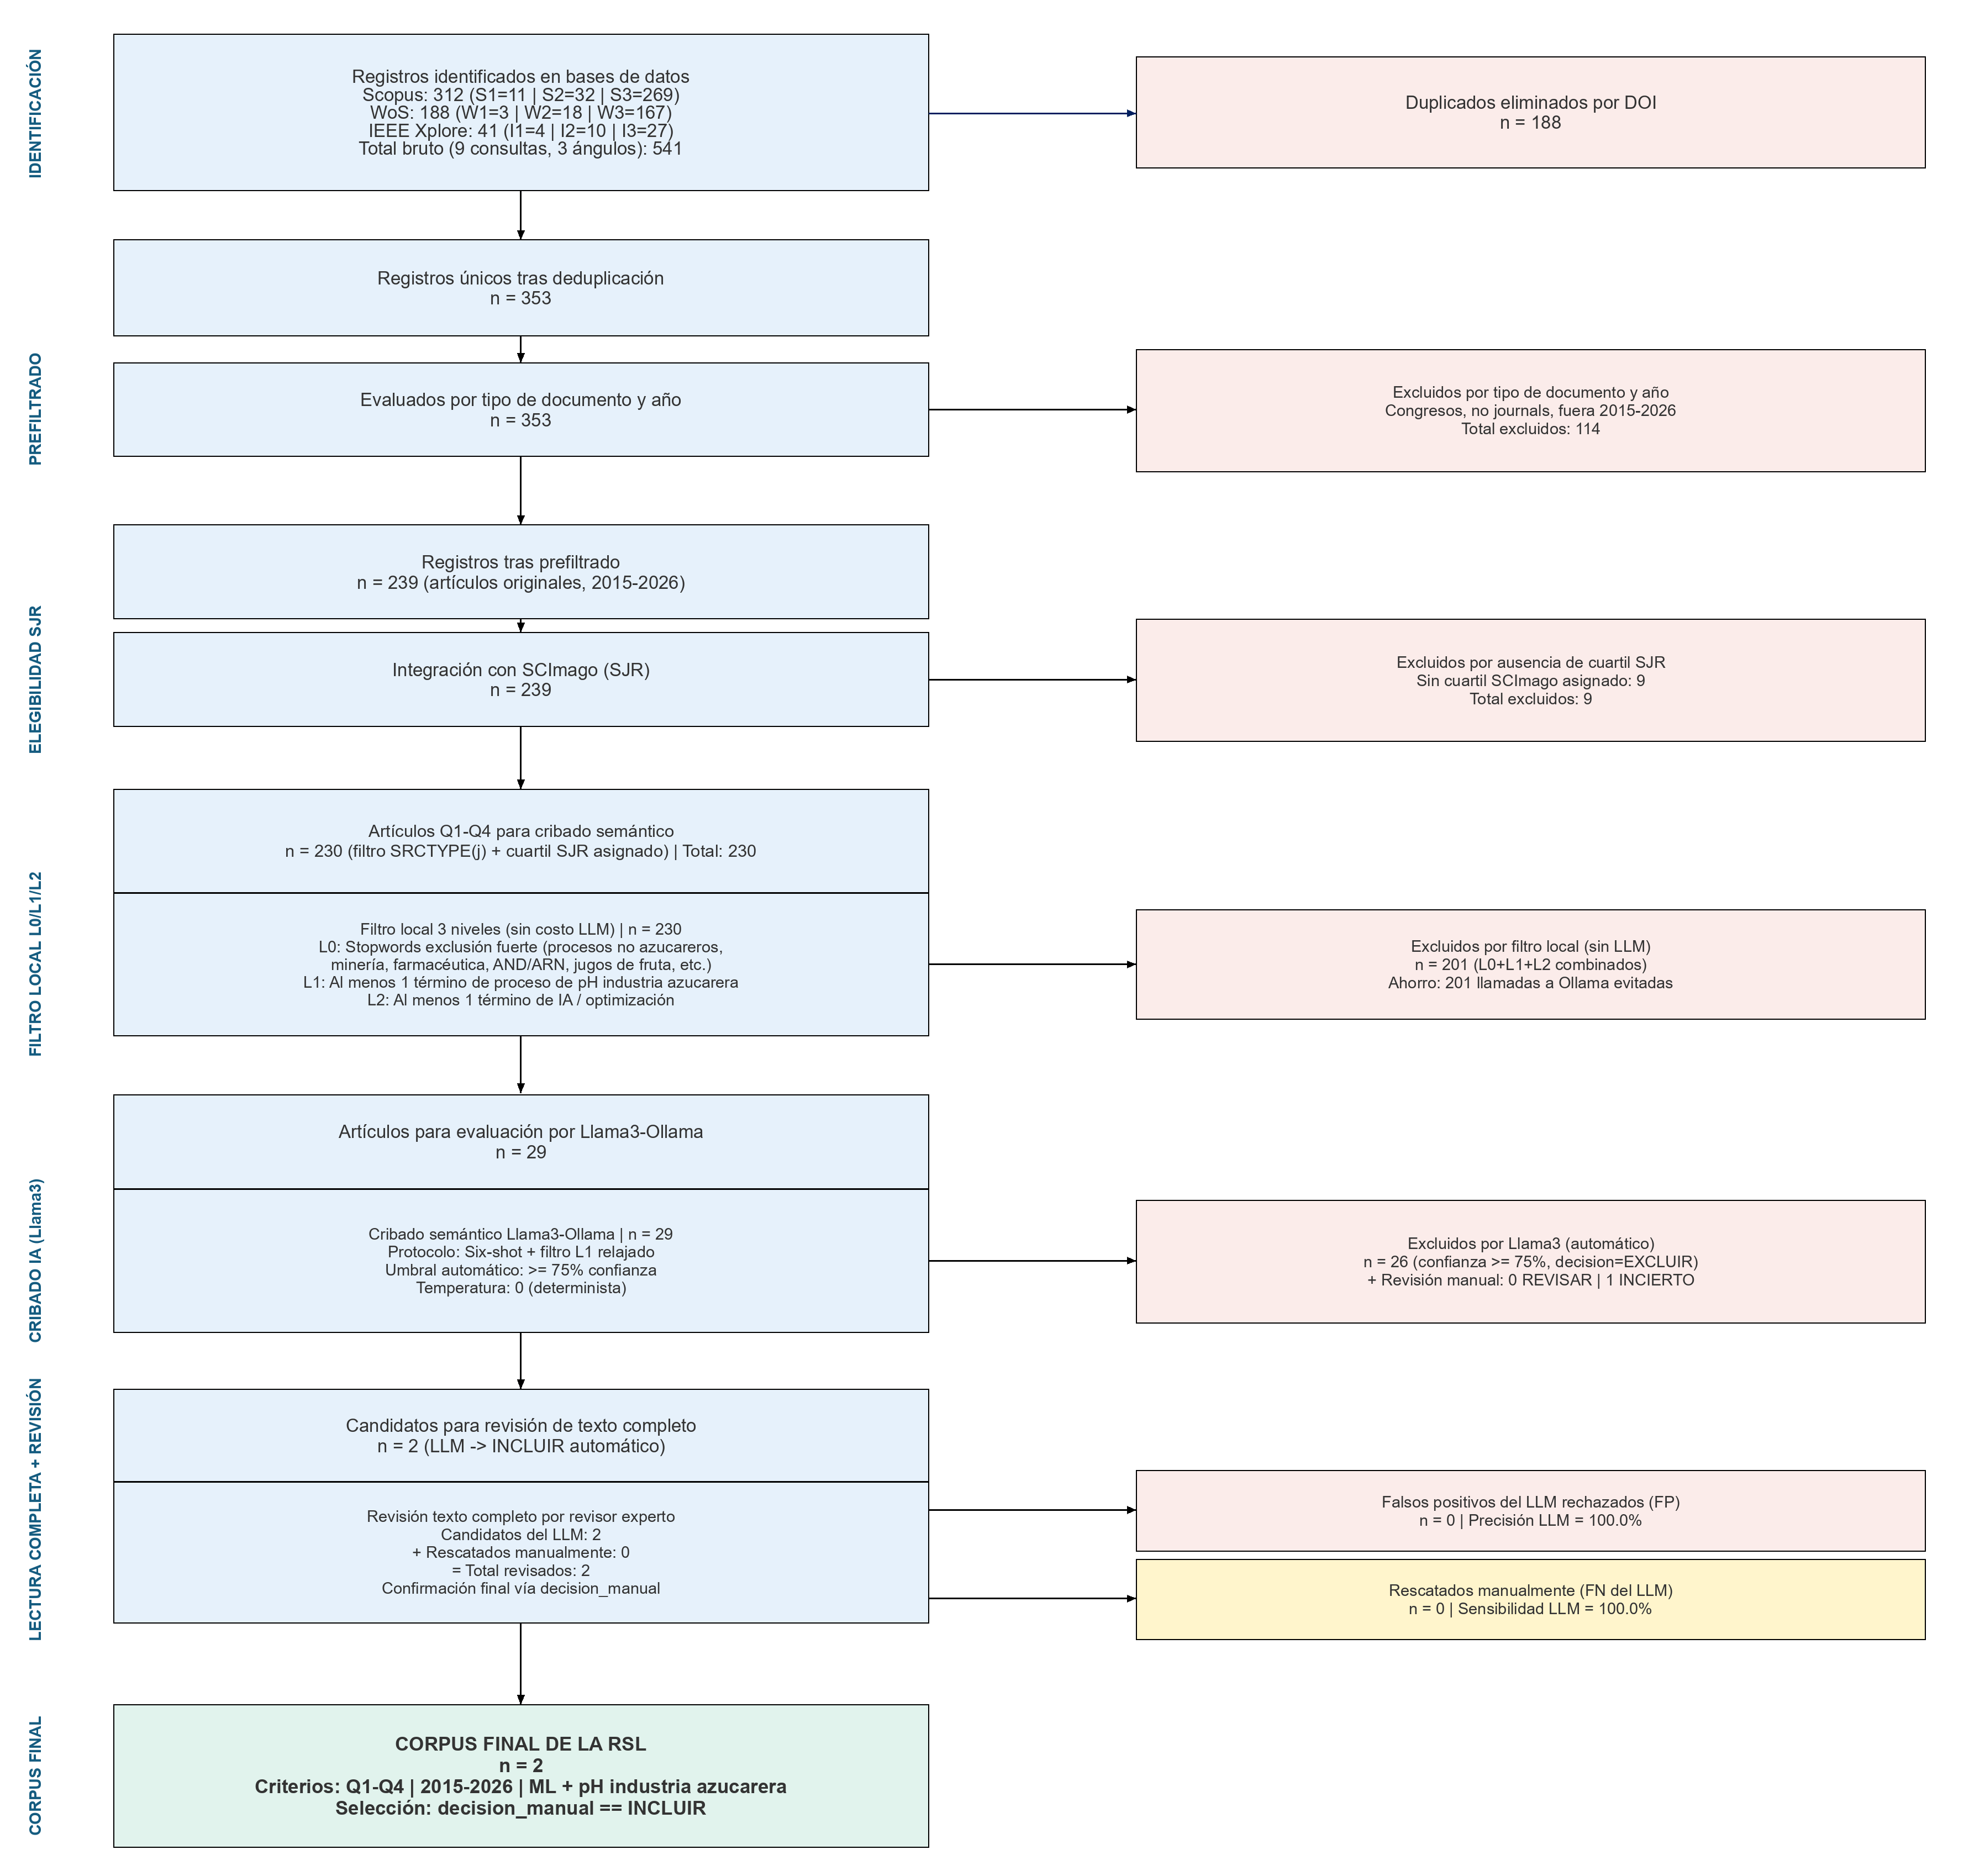
\includegraphics[width=0.9\textwidth,height=1\textheight,keepaspectratio]{Diagrama_RSL.png}
\begin{Nota}[Nota]{0.9\textwidth}{Elaboración propia. Adaptado de
PRISMA-ScR \parencite{tricco2018prismascr}. Búsqueda ejecutada el
\FechaBusqueda; filtro de cuartil y cribado ejecutados en septiembre de
2026. La verificación léxica y el análisis de sensibilidad
(\ref{sub:sensibilidad}) no alteran el embudo.}
\end{Nota}
\end{figure}
\linenumbers

\subsection{Fiabilidad del cribado}
\label{sub:res_kappa}

\textbf{Métrica primaria: $\kappa$ inter-humano.} Sobre los
230~registros, la concordancia entre los Revisores~1 y~2 fue
$\kappa_{\text{inter}}=$\,\KappaInter, con concordancia observada
\PzeroInter{} (Tabla~\ref{tab:confusion_inter}): no hubo ninguna
discrepancia, de modo que la decisión consensuada coincide con la de
ambos revisores. Respecto del consenso, la sensibilidad fue \SensInter,
la precisión \PrecInter{} y $F_1=$\,\FUnoInter, con IC 95\,\% de Wilson
\ICInter; $\text{PABAK}_{\text{inter}}=$\,\PABAKInter.
El corpus contiene \NPositivosMuestra{} registros positivos (prevalencia
\PrevInter): con tan pocos positivos el intervalo de la sensibilidad es
amplio, y un $\kappa$ o PABAK máximos reflejan sobre todo la baja
prevalencia y la facilidad de excluir los 228~registros claramente
ajenos al tema, no concordancia sobre casos dudosos; el resultado debe
leerse como estimación de la fiabilidad del proceso de exclusión y no
como evidencia de desempeño sobre casos positivos. Una concordancia
perfecta sin discrepancias, además, no permite estimar la variabilidad
entre revisores.

\nolinenumbers
\begin{table}[H]
\centering
\caption{Matriz de confusión \textbf{inter-humano} (Revisor~1 vs.\
Revisor~2) sobre los 230~registros del corpus Q1--Q4. Métrica primaria
de fiabilidad del cribado.}
\label{tab:confusion_inter}
\begin{tblr}{colspec={X[4.2]X[2.4]X[2.4]X[0.9]},width=0.9\textwidth,stretch=1,
  hline{1,2,Z}={0.8pt},row{1,Z}={font=\bfseries}}
 & Revisor~2 INCLUIR & Revisor~2 EXCLUIR & Total \\
Revisor~1 INCLUIR & \VPInter~\textsf{[VP]} & \FNInter~\textsf{[FN]} & \TotUnoI \\
Revisor~1 EXCLUIR & \FPInter~\textsf{[FP]} & \VNInter~\textsf{[VN]} & \TotUnoE \\
Total & \TotDosI & \TotDosE & 230 \\
\end{tblr}
\begin{Nota}[Nota]{0.9\textwidth}{VP: verdaderos positivos; VN: verdaderos
negativos; FP: falsos positivos; FN: falsos negativos. $P_0=$\,\PzeroInter;
$\kappa_{\text{inter}}=$\,\KappaInter; $\text{PABAK}=$\,\PABAKInter.}
\end{Nota}
\end{table}
\linenumbers

\textbf{Métrica secundaria: concordancia con el \textit{pipeline}
automático.} En la corrida de producción el \textit{pipeline} coincidió
con la decisión humana final en los 230~registros ($\kappa=1.000$). Sin
embargo, esa cifra no es reproducible: al re-ejecutar los 29~registros
que llegan al modelo con el mismo modelo, $T=0$ y el \textit{prompt}
original, el modelo clasificó como INCLUIR un tercer registro (un estudio
de clarificación de jugo con peróxido de hidrógeno y redes neuronales que
la decisión humana final excluyó), lo
que da 229/230 coincidencias ($\kappa=0.798$, $\text{PABAK}=0.991$).
Con el \textit{prompt} corregido, sin la fuga de información, el
resultado fue idéntico (3~INCLUIR, 229/230), y el estudio de
\cite{palaciomorales2021optimiza} se mantuvo como INCLUIR (confianza
$95\to98\,\%$): la fuga no determinó su clasificación. El detalle está
en el Apéndice~\ref{apx:kappa_notas}.

\subsection{Los estudios incluidos}
\label{sub:res_estudio}

Los dos estudios (Tabla~\ref{tab:studies}) abordan la regulación del pH
en la clarificación del jugo con técnicas de control inteligente y
optimización. \cite{palaciomorales2021optimiza}, en \textit{Processes}
(MDPI; Q2 SJR~2024), formula un NMPC cuyo modelo interno es un sistema
difuso Takagi--Sugeno identificado y cuyos parámetros se sintonizan con
una búsqueda de patrón sin gradiente; se evalúa sobre un modelo de planta
\textit{simulado} de invariantes de reacción y se compara con otras cinco
sintonías de NMPC publicadas (no con un PID), con mejor índice ICET pero
sobreimpulso equivalente y mayor esfuerzo de control que cuatro de ellas.
\cite{murugesan2020computeraided}, en \textit{Circuits, Systems, and
Signal Processing} (Springer; Q3 SJR~2024), identifica un modelo de
segundo orden del clarificador a partir de 3000~muestras reales de una
planta y sintoniza fuera de línea un PID con un algoritmo de transición de
estado, comparado con GA y PSO, con menor MSE y tiempo de asentamiento
pero sin ventaja en el tiempo de subida. Ninguno implementó el control en
lazo cerrado en planta (TRL~$\approx 3$--$4$); ambos usan optimización
sin gradiente para sintonizar o identificar. El riesgo de sesgo
(Apéndice~\ref{apx:herramienta_sesgo}) fue moderado--alto para
\cite{palaciomorales2021optimiza} y moderado para
\cite{murugesan2020computeraided}.

% Tabla de caracterización de los dos estudios incluidos (apaisada).
% Datos extraídos del TEXTO COMPLETO (04_corpus_final/pdfs/), no del resumen.
\newgeometry{margin=2cm}
\begin{landscape}
\sloppy
\hfuzz=500pt
\emergencystretch=3em
\begin{longtblr}[
caption={\textit{Caracterización de los dos estudios incluidos, extraída del
texto completo. Las cifras corresponden a la comparación intra-estudio
reportada por los autores; no constituyen una síntesis entre estudios.}},
label={tab:studies},
]{colspec={X[1.2]X[1.7]X[3.0]X[3.0]X[3.6]X[3.3]},width=1.0\linewidth,
  hline{1,2,Z}={0.6pt},row{1}={font=\bfseries}}
Estudio & Objetivo & Estrategia de modelado y control &
Datos y variables & Resultados clave (intra-estudio) &
Validación y limitaciones \\
\cite{palaciomorales2021optimiza}
& Sintonizar un NMPC para regular el pH en la alcalinización del jugo de
  caña (\textit{setpoint} 7.34) tras identificar su modelo interno
& Modelo interno Takagi--Sugeno de entrada--salida con conjuntos difusos
  multidimensionales (consecuentes lineales); identificación y sintonía del
  NMPC (horizontes y pesos) mediante búsqueda de patrón generalizada, sin
  gradiente
& Planta \textbf{simulada} con un modelo de invariantes de reacción
  (HNO$_3$ + NaHCO$_3$) tomado de una tesis doctoral, no datos de planta.
  Manipulada: caudal de lechada de cal $F_2$ (10--70~GPM).
  Perturbaciones: caudal de jugo sulfitado $F_1$ (500--2100~GPM) y pH del
  jugo sulfitado y de la lechada. Salida: pH del jugo alcalinizado
  (5.7--8.7)
& Índice ICET(pH) $=553$ frente a $2.41$--$3.95\times10^{3}$ de otras cinco
  sintonías de NMPC publicadas (menor es mejor). Sobreimpulso
  $M_p=30.3\,\%$ frente a $29.8$--$31.1\,\%$ (sin mejora). Esfuerzo de
  control $79.2$ frente a $28.0$--$83.4$ (mayor que el de cuatro de las
  cinco). \textbf{No se compara con un PID/PI}
& Solo \textbf{simulación} (TRL~$\approx 3$--$4$, escala NASA
  NPR~7123.1B); sin planta piloto ni industrial. Los autores reportan
  rizado residual en la respuesta; el modelo de planta es un
  \textit{benchmark} genérico, no un clarificador medido \\
\cite{murugesan2020computeraided}
& Estimar los parámetros del modelo del clarificador y sintonizar fuera
  de línea un controlador PID para la neutralización del pH
& Identificación estándar (modelo de segundo orden) refinada con un
  \textit{state transition algorithm} con restricciones lagrangianas
  (LSTA); sintonía de $K_p$, $T_i$, $T_d$ minimizando el MSE; comparación
  con GA y PSO
& \textbf{Datos reales de planta} (M/S Sakthi Sugars Ltd.): 3000 muestras en
  dos turnos, 70\,\% entrenamiento y 30\,\% prueba. Entrada: caudal de
  lechada de cal. Salida: pH final del jugo
& MSE $1.2\times10^{-3}$ (LSTA) frente a $3.3\times10^{-2}$ (GA) y
  $6.6\times10^{-1}$ (PSO); tiempo de asentamiento $46.1$~s frente a $52.2$ y
  $94.8$~s; tiempo de subida $33.4$~s (LSTA) frente a $28.3$ (GA) y $37.4$~s
  (PSO), sin ventaja de LSTA en este índice
& Identificación \textbf{fuera de línea con datos de planta}; el
  controlador solo se evalúa en \textbf{simulación} (respuesta a escalón),
  sin implementación en lazo cerrado (TRL~$\approx 4$). Modelo lineal de
  segundo orden para un proceso no lineal; el controlador es PID
  sintonizado por metaheurística \\
\end{longtblr}
\nolinenumbers
\begin{Nota}[Nota]{\linewidth}{Elaboración propia a partir del texto
completo de \cite{palaciomorales2021optimiza} (DOI: 10.3390/pr9122283) y
\cite{murugesan2020computeraided} (DOI: 10.1007/s00034-019-01139-5).
Abreviaturas: NMPC $=$ \textit{nonlinear model predictive control};
ICET $=$ integral del error cuadrático ponderado por el tiempo; GA
$=$ algoritmo genético; PSO $=$ optimización por enjambre de partículas;
TRL $=$ \textit{technology readiness level}
\parencite{nasa2016trl}. Las cifras se citan tal como las reportan los
autores originales.}
\end{Nota}
\nolinenumbers
\end{landscape}
\restoregeometry

\linenumbers

\subsection{Evidencia \textit{in-domain} excluida por criterios formales}
\label{sub:res_complementaria}

El análisis de sensibilidad (\ref{sub:sensibilidad}) identificó
11~trabajos que comparten con los incluidos el proceso (neutralización o
clarificación del jugo azucarero), la variable (pH) y el uso de control
avanzado o AA, pero que no cumplen los criterios formales: 3~artículos en
revistas sin cuartil en SCImago~2024 y 8~actas o capítulos de series de
libros (Apéndice~\ref{apx:complementaria}, Tabla~F1). Se caracterizan de
forma descriptiva a partir de sus resúmenes, no entran en el corpus
incluido ni en el cálculo de $\kappa$, y la Figura~\ref{fig:evidencia}
los sitúa junto a los dos incluidos. Un registro adicional sobre la
defecosaturación de jugo de remolacha con una red neuronal
\parencite{vlasenko2023neural} no se contabiliza porque el pH es variable
de entrada y no objetivo (criterio de exclusión~e).

\nolinenumbers
\begin{figure}[H]
\centering
\captionsetup{width=0.95\textwidth}
\caption{Mapa de evidencia \textit{in-domain} sobre pH de la
clarificación azucarera: los 2~estudios incluidos y los 11~trabajos
excluidos por criterios formales, según familia de método y nivel de
validación declarado.}
\label{fig:evidencia}
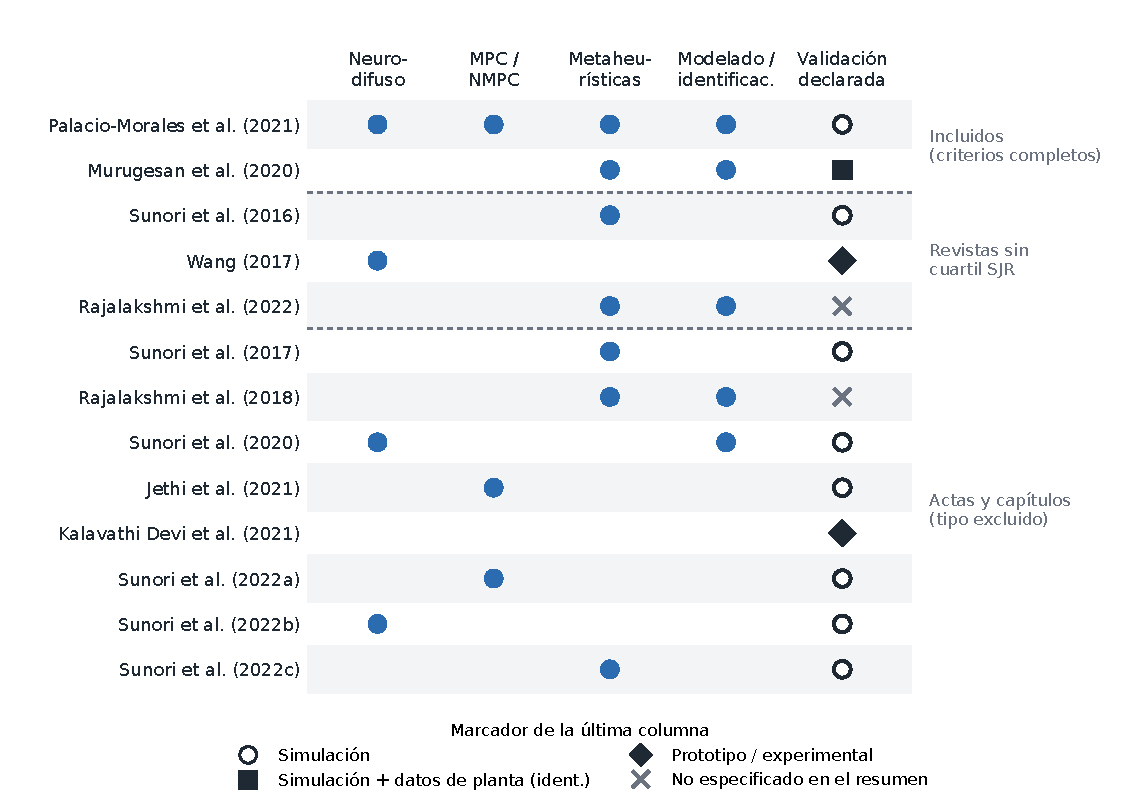
\includegraphics[width=0.95\textwidth]{mapa_evidencia.pdf}
\begin{Nota}[Nota]{0.95\textwidth}{Elaboración propia. Los dos incluidos se
clasificaron con el texto completo; los 11~complementarios, solo con el
resumen, por lo que ``no especificado'' indica que el resumen no declara
el nivel de validación. Una fila puede aparecer en varias familias.
Referencias completas en la Tabla~F1 (Apéndice~\ref{apx:complementaria}).}
\end{Nota}
\end{figure}
\linenumbers

Tres rasgos caracterizan este conjunto de 13~trabajos
(2016--2022): (i)~\textbf{validación mayoritariamente en simulación}: de
los 11 complementarios, 7 son simulaciones, 2 declaran prototipo o
resultados experimentales sin precisar su escala
\parencite{wang2017ph,kdt2021sensor} y 2 no especifican el nivel en el
resumen; ninguno declara control en lazo cerrado en una planta
industrial; (ii)~\textbf{ausencia de aprendizaje por refuerzo y de
sensores virtuales} de pH para uso en línea, pues el AA aparece solo como
modelado (SVR, redes, ANFIS) o como optimizador; y (iii)~\textbf{alta
concentración autoral}: 10 de los 13 trabajos proceden de dos grupos de
autores (7 del grupo Sunori--Juneja y 3 del grupo
Rajalakshmi--Jeyadevi--Karthik, que incluye a
\cite{murugesan2020computeraided}). Ningún trabajo \textit{in-domain}
identificado es posterior a 2022.

\subsection{Caracterización bibliométrica del campo adyacente}
\label{sub:res_biblio}

El corpus Q1--Q4 (230~registros) crece de forma sostenida, con
aceleración desde 2022: los años 2023--2026 concentran 118~registros
(51.3\,\%), y los 25~de 2026 son publicaciones \textit{early access}
(Figura~\ref{fig:produccion}). Las revistas más frecuentes son de ciencia
y tecnología de alimentos (\textit{LWT} $n=6$; \textit{Food Chemistry}
$n=5$; \textit{Bioresource Technology} $n=5$; \textit{Journal of Food
Process Engineering} $n=4$; \textit{Biomass Conversion and
Biorefinery} $n=4$), sin presencia dominante de revistas de teoría de
control.

\nolinenumbers
\begin{figure}[H]
\centering
\captionsetup{width=0.8\textwidth}
\caption{Producción anual del corpus adyacente Q1--Q4 ($n=230$;
2015--2026).}
\label{fig:produccion}
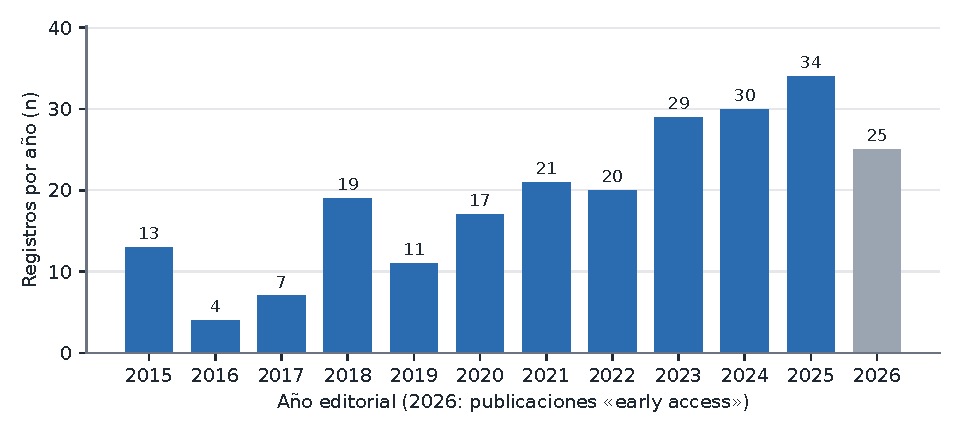
\includegraphics[width=0.78\textwidth]{produccion_anual.pdf}
\begin{Nota}[Nota]{0.8\textwidth}{Elaboración propia a partir de
\texttt{3.filtrado\_quartiles.xlsx}. El crecimiento refleja el campo
adyacente, no la regulación de pH del proceso azucarero, cuyos trabajos
\textit{in-domain} no superan el año 2022 (\ref{sub:res_complementaria}).}
\end{Nota}
\end{figure}
\linenumbers

La red de co-ocurrencia (120~nodos, 2403~aristas, densidad $0.337$)
identificó cuatro comunidades por Louvain (Figura~\ref{fig:vos};
Tabla~\ref{tab:comunidades}). Las etiquetas automáticas del
\textit{pipeline}, orientadas \textit{a~priori} a las RQ, no describían
los términos que dominan cada comunidad y se corrigieron por contenido
real. La red incluye términos indexados por las bases (p.~ej.\
\textit{nonhuman}, \textit{controlled study}, \textit{unclassified drug}),
ruido de indexación que impide leerla como mapa temático fino; por eso
se usa para \emph{caracterizar} el campo adyacente y no como prueba de
la brecha, que descansa en el embudo (\ref{sub:res_prisma}) y en la
verificación léxica (\ref{sub:res_mapeo}).

\nolinenumbers
\begin{figure}[H]
\centering
\captionsetup{width=0.9\textwidth}
\caption{Red de co-ocurrencia de palabras clave del corpus adyacente
Q1--Q4 ($n=230$; umbral $\geq 2$; comunidades por Louvain). Ninguna de
las cuatro comunidades corresponde a la intersección
\{AA/control avanzado\,$\times$\,pH\,$\times$\,industria azucarera\}.}
\label{fig:vos}
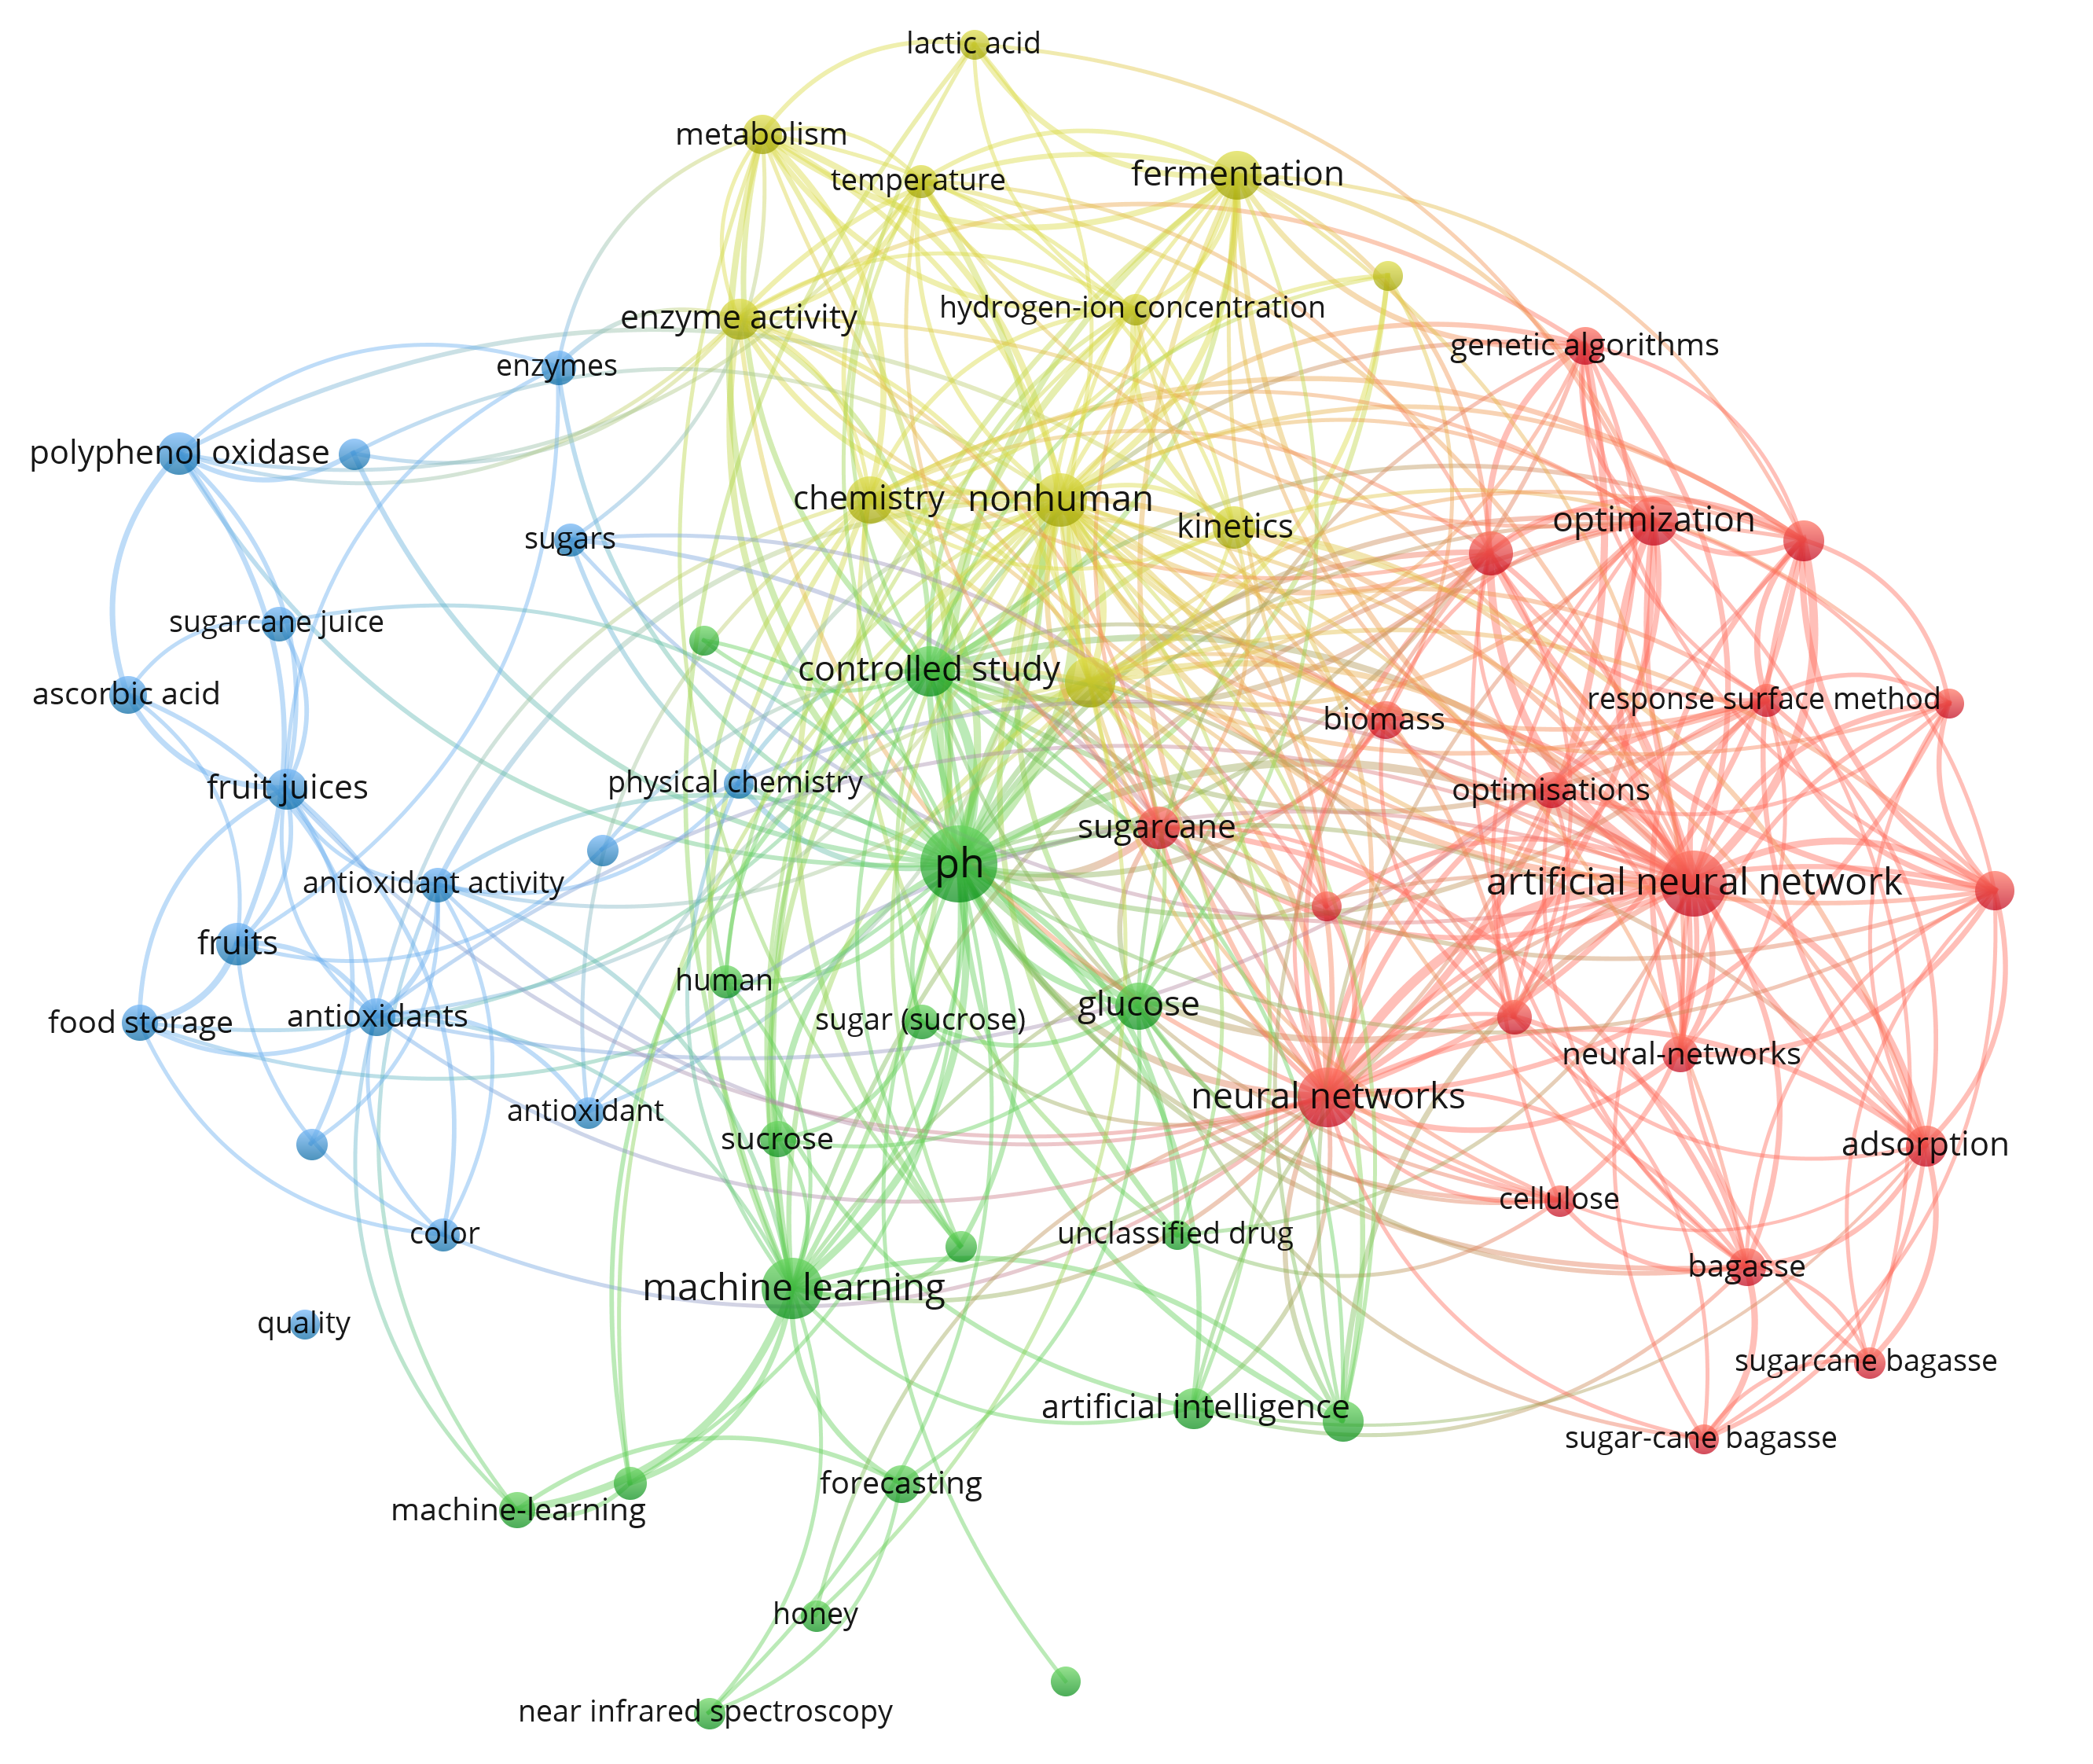
\includegraphics[width=0.85\textwidth,height=0.65\textheight,keepaspectratio]{fitrado_quartiles.png}
\begin{Nota}[Nota]{0.9\textwidth}{Elaboración propia con
\textit{bibliometrix} \parencite{ARIA2017959} y \textit{VOSviewer}
\parencite{vanecksoftware2010}. El tamaño del nodo indica la frecuencia
del término y el grosor de los enlaces la fuerza de co-ocurrencia. El
vocabulario de los dos estudios incluidos (\textit{pH neutralization},
\textit{clarifier process}) tiene frecuencia 1 y queda bajo el umbral.}
\end{Nota}
\end{figure}
\begin{table}[H]
\centering
\caption{Comunidades temáticas detectadas por Louvain sobre la red de
co-ocurrencia del corpus Q1--Q4 ($n=230$). Etiquetas corregidas por
contenido dominante.}
\label{tab:comunidades}
\small
\begin{tblr}{colspec={X[0.5]X[3.3]X[5.5]X[0.9]X[0.9]},width=\textwidth,
  hline{1,2,Z}={0.6pt},row{1}={font=\bfseries}}
\# & Etiqueta (por contenido real) & Términos dominantes
  & $N^{\circ}$ térm. & Frec. \\
C1 & Modelado ANN/GA/RSM y valorización de bagazo (optimización numérica
  de procesos) &
  neural network, artificial neural network, genetic algorithm,
  optimization, sugarcane, response surface methodology, adsorption,
  bagasse, biomass, cellulose, scanning electron microscopy,
  lignocellulose, saccharum & 47 & 455 \\
C2 & ML/quimiometría para calidad de jugos y alimentos &
  fruits, polyphenol oxidase, fruit juices, juice quality, antioxidants,
  food storage, antioxidant activity, color, peroxidase,
  physicochemical properties, total soluble solids, shelf life & 28 & 242 \\
C3 & Bioprocesos, cinética enzimática y química del azúcar &
  sugar, fermentation, prediction, kinetics, metabolism, enzymes,
  sugars, hydrogen-ion concentration, lactic acid, nitrogen,
  biosynthesis, substrate concentration & 16 & 178 \\
C4 & Métodos de AA generales y espectroscopía no destructiva &
  machine learning, artificial intelligence, forecasting, sucrose,
  near infrared spectroscopy, honey, support vector machines,
  deep learning, chemometrics, random forest,
  partial least squares regression, principal component analysis
  & 29 & 239 \\
\end{tblr}
\begin{Nota}[Nota]{\textwidth}{Elaboración propia. Ninguna comunidad
corresponde a la intersección \{AA/control avanzado\,$\times$\,pH\,$\times$\,industria
azucarera\}. El campo se organiza en torno a optimización numérica de
modelos y valorización de bagazo (C1), calidad de jugos (C2), bioquímica
y cinética enzimática (C3) y métodos generales de AA aplicados a
espectroscopía (C4).}
\end{Nota}
\end{table}
\linenumbers

\subsection{Verificación léxica y mapeo frente a las preguntas de investigación}
\label{sub:res_mapeo}

La Tabla~\ref{tab:auditoria} combina las dos líneas de evidencia léxica:
el conteo sobre los 353~registros únicos (verificación independiente del
umbral $\geq 2$) y la presencia en la red del corpus Q1--Q4. Los términos
de aprendizaje por refuerzo no aparecen en ningún registro; \textit{soft
sensor} aparece en 5~registros, ninguno en contexto azucarero; y MPC/NMPC
aparece en 5, de los cuales 4 son los ya identificados en
\ref{sub:res_estudio} y \ref{sub:res_complementaria}. El vacío que
indicaba la red a umbral $\geq 2$ se confirma sin umbral, pero la
verificación también muestra que el vocabulario de control avanzado
\emph{sí} existe en los registros \textit{in-domain} excluidos por
criterios formales.

\nolinenumbers
\begin{table}[H]
\centering
\caption{Verificación léxica de los conceptos núcleo de las RQ en los
353~registros únicos (título, resumen y palabras clave) y su presencia en
la red del corpus Q1--Q4.}
\label{tab:auditoria}
\small
\begin{tblr}{colspec={X[3.2]X[1.2]X[1.0]X[1.4]X[1.4]X[2.0]},width=\textwidth,
  hline{1,2,Z}={0.6pt},row{1}={font=\bfseries}}
Concepto núcleo & Registros & + pH & + proceso azucarero & + pH y proceso azucarero & En la red Q1--Q4 (frec.~$\geq 2$) \\
Sensor virtual / \textit{soft sensor} & 5 & 5 & 0 & 0 & Ausente \\
MPC / NMPC & 5 & 5 & 4 & 4 & Ausente \\
Aprendizaje por refuerzo & 0 & 0 & 0 & 0 & Ausente \\
PID / PI & 5 & 5 & 4 & 4 & Ausente \\
Control difuso / neuro-difuso & 16 & 16 & 8 & 8 & Marginal \\
Metaheurísticas & 45 & 45 & 12 & 12 & Presente (optimización) \\
Control adaptativo / \textit{gain scheduling} & 2 & 2 & 1 & 1 & Ausente \\
Gemelo digital & 1 & 1 & 0 & 0 & Ausente \\
Redes neuronales / AA general & 221 & 210 & 28 & 25 & Abundante \\
\end{tblr}
\begin{Nota}[Nota]{\textwidth}{Elaboración propia (\texttt{12\_auditoria\_conceptual.py}).
``Proceso azucarero'' agrupa expresiones como \textit{sugar mill},
\textit{juice clarification}, \textit{cane juice} o \textit{sugar beet};
``pH'' incluye neutralización, alcalinización y encalado. Del total de
353~registros, 64 combinan pH y proceso azucarero. Los términos de las
palabras clave incluyen descriptores indexados por la base.}
\end{Nota}
\end{table}
\linenumbers

Traducido a las preguntas de investigación (Tabla~\ref{tab:mapeo_rqs}),
la evidencia es más densa de lo que sugería el corpus estricto en RQ1 y
RQ2, pero poco madura en las tres.

\nolinenumbers
\begin{table}[H]
\centering
\caption{Estado de la evidencia por pregunta de investigación
(corpus incluido y evidencia complementaria).}
\label{tab:mapeo_rqs}
\small
\begin{tblr}{colspec={X[0.6]X[5.2]X[2.2]},width=\textwidth,
  hline{1,2,Z}={0.6pt},row{1}={font=\bfseries}}
RQ & Evidencia \textit{in-domain} (incluidos y complementarios) & Estado \\
RQ1 & Identificación con datos de planta
  \parencite{murugesan2020computeraided}; modelos T--S, SVR y ANFIS sobre
  modelos simulados o sin datos declarados; ningún sensor virtual de pH
  para operación en línea & Evidencia parcial; madurez baja \\
RQ2 & NMPC \parencite{palaciomorales2021optimiza}, MPC y $H_\infty$ frente
  a PID, ANFIS frente a PI y PID sintonizado por metaheurísticas,
  casi siempre en simulación sobre modelos de función de transferencia;
  sin comparación en planta & Evidencia existente; \textbf{brecha de
  validación} \\
RQ3 & AA como modelado u optimizador; aprendizaje por refuerzo ausente;
  ningún estudio analiza barreras de adopción industrial &
  \textbf{Brecha mayor} \\
\end{tblr}
\end{table}
\linenumbers

% ─────────────────────────────────────────────────────────────────────────────
\section{Discusión}
\label{sec:discusion}
% ─────────────────────────────────────────────────────────────────────────────

\subsection{Interpretación de la brecha}
\label{sub:interpretacion}

El hallazgo central es una \textbf{brecha cualificada}, no una ausencia de
investigación. El corpus que cumple todos los criterios es de dos
estudios, pero el análisis de sensibilidad muestra que existen al menos
once trabajos más sobre el mismo problema, publicados en actas y en
revistas sin cuartil. Lo que falta no es investigación sobre control
avanzado del pH azucarero sino su \emph{madurez y diversidad}: casi todo
se valida en simulación sobre modelos de función de transferencia, no hay
aprendizaje por refuerzo ni sensores virtuales operativos, no se
documenta una línea base de PID en planta con la que medir la mejora, y
la producción se concentra en dos grupos y no supera 2022, mientras el
campo adyacente se acelera (51.3\,\% de los registros en 2023--2026).
Un corpus mínimo bajo un protocolo auditable es informativo por sí mismo
\parencite{yaffe2012empty,lang2007empty}, pero solo si se acompaña de lo
que aquí se hizo: reportar de forma explícita qué evidencia queda fuera
por diseño y cuánto cambia la conclusión al incluirla.

Se examinaron explicaciones alternativas. \emph{(a)~Nicho demasiado
estrecho; la transferencia directa basta.} Los propios estudios
muestran que la transferencia \emph{ya ocurrió en simulación}: el modelo
de planta de \cite{palaciomorales2021optimiza} es un \textit{benchmark}
de neutralización de invariantes de reacción
\parencite{gustafsson1983dynamic} y no un jugo de caña medido. Lo que
no se ha demostrado es que los métodos funcionen con las particularidades
del jugo (coloides, varios ácidos débiles, \textit{fouling}); la brecha es
empírica y de validación, no conceptual. \emph{(b)~El conocimiento
existe, pero en canales de baja visibilidad.} Es coherente con la
concentración en actas y en dos grupos. \emph{(c)~La práctica industrial
no se publica.} Es plausible y no puede evaluarse con literatura
indexada; se declara como limitación.

\subsection{Métodos transferibles desde dominios vecinos}
\label{sub:transferibilidad}

La analogía dinámica es el punto de partida: la curva de titulación del
jugo comparte con la neutralización ácido--base genérica una ganancia
variable en torno al punto de equivalencia \parencite{shinskey1996process}.
La Tabla~\ref{tab:transferibilidad} sintetiza, por familia de método, la
evidencia de dominios vecinos, la evidencia \textit{in-domain} hallada en
esta revisión, la barrera principal y el horizonte propuesto.

\nolinenumbers
\begin{table}[H]
\centering
\caption{Matriz de transferibilidad de familias de métodos al encalado
azucarero.}
\label{tab:transferibilidad}
\small
\begin{tblr}{colspec={X[1.5]X[2.6]X[1.9]X[2.4]X[1.0]},width=\textwidth,
  hline{1,2,Z}={0.6pt},row{1}={font=\bfseries}}
Familia & Dominios vecinos & \textit{In-domain} (de 13) & Barrera principal en el encalado & Horizonte \\
Control difuso / neuro-difuso &
  \cite{herediamolinero2014feedback,suguna2026advanced} &
  4 (modelo T--S, ANFIS, PID difuso) &
  Validación en lazo cerrado con datos reales; deriva del electrodo & Corto \\
Sensores virtuales / \textit{data-driven} &
  \cite{son2021deep,xu2022datadriven,bardeeniz2025artificial} &
  4 como modelado; 0 operativos &
  Datos etiquetados escasos; \textit{fouling} y baja frecuencia de
  laboratorio & Corto \\
Metaheurísticas (identificación y sintonía) &
  No revisada (fuera del alcance de esta revisión) &
  7 &
  Optimización fuera de línea sobre modelos simplificados; sin
  resintonía en línea & Corto \\
MPC / NMPC y caja gris &
  \cite{henson1994adaptive,berenguel2004model,durairaj2023deep,otalora2026enhancing} &
  3 &
  Modelo fiel con composición variable; costo de cómputo & Mediano \\
Aprendizaje por refuerzo &
  \cite{alvesgoulart2020autonomous,panjapornpon2022reinforcement} &
  0 &
  Datos y exploración segura; requiere gemelo digital previo & Largo \\
\end{tblr}
\begin{Nota}[Nota]{\textwidth}{Elaboración propia. Una referencia puede
pertenecer a varias familias; los conteos \textit{in-domain} provienen
de la Figura~\ref{fig:evidencia}. La selección de dominios vecinos es
ilustrativa y no sistemática.}
\end{Nota}
\end{table}
\linenumbers

En el eje del \textbf{control predictivo}, el linaje que va de la
identificación no lineal en tiempo real \parencite{proll1994modelpredictive}
y el control adaptativo basado en invariantes de reacción
\parencite{henson1994adaptive} hasta los esquemas recientes con
identificación por aprendizaje profundo \parencite{durairaj2023deep}
indica que el NMPC es viable si se dispone de un modelo suficientemente
fiel, condición onerosa en el jugo de caña; los dos estudios incluidos
abordan esa condición con identificación explícita, lo que motiva
enfoques de caja gris que combinen invariantes de reacción con ajuste
\textit{data-driven}. En el eje del \textbf{control inteligente}, los
controladores difusos y neuro-difusos diseñados para operar cerca del
punto de equivalencia \parencite{herediamolinero2014feedback,suguna2026advanced}
son pertinentes porque abordan la región de máxima sensibilidad. En el eje
del \textbf{aprendizaje por refuerzo}, las políticas autónomas
demostradas en efluentes y procesos multivariables
\parencite{alvesgoulart2020autonomous,panjapornpon2022reinforcement}
requieren volúmenes de datos y exploración que chocan con la escasez de
datos históricos etiquetados y con las restricciones operativas de un
ingenio. Los \textbf{sensores virtuales}
\parencite{son2021deep,xu2022datadriven,bardeeniz2025artificial} ofrecen
una vía de menor riesgo frente al \textit{fouling}. La transferibilidad no
es uniforme: los enfoques difusos y los sensores virtuales son los de
adopción más plausible a corto plazo; el NMPC exige resolver antes el
modelado; y el aprendizaje por refuerzo depende de una infraestructura
de datos aún inexistente en el sector.

\subsection{Agenda de investigación}
\label{sub:agenda}

La agenda se organiza en tres horizontes y una condición habilitante
previa (Figura~\ref{fig:hoja_ruta}).

\nolinenumbers
\begin{figure}[H]
\centering
\captionsetup{width=0.95\textwidth}
\caption{Hoja de ruta propuesta por horizontes de madurez tecnológica
(TRL), con las condiciones habilitantes transversales.}
\label{fig:hoja_ruta}
\resizebox{0.95\textwidth}{!}{% hoja_ruta.tex — Hoja de ruta por horizontes TRL (figura propia, TikZ).
% Se incluye vía \input{} en 04_body.tex (§ Agenda de investigación).
\begin{tikzpicture}[
  font=\sffamily\scriptsize,
  hz/.style = {draw, rounded corners=3pt, align=left, text width=4.3cm,
               inner sep=5pt, line width=0.6pt, minimum height=3.6cm,
               anchor=north},
  corto/.style = {hz, fill=green!7},
  medio/.style = {hz, fill=blue!7},
  largo/.style = {hz, fill=orange!9},
  cab/.style = {font=\sffamily\bfseries\scriptsize, align=center},
  base/.style = {draw, rounded corners=3pt, fill=black!5, align=center,
                 text width=14.6cm, inner sep=5pt, line width=0.6pt},
  flecha/.style = {-{Stealth[length=2.2mm]}, line width=0.9pt, black!60},
]

% ── Cabeceras ──────────────────────────────────────────────────────────────
\node[cab] at (2.4, 5.0)  {Corto plazo\\TRL 4--5};
\node[cab] at (7.6, 5.0)  {Mediano plazo\\TRL 5--6};
\node[cab] at (12.8, 5.0) {Largo plazo\\TRL 7--8};

% ── Horizontes ─────────────────────────────────────────────────────────────
\node[corto] (c) at (2.4, 4.4) {%
  \textbf{Control neuro-difuso}\\ réplica en banco con jugo real;\\[2pt]
  \textbf{Sensores virtuales de pH}\\ entrenados con variables DCS de bajo
  costo, robustos al \textit{fouling}};
\node[medio] (m) at (7.6, 4.4) {%
  \textbf{NMPC de caja gris}\\ invariantes de reacción + identificación en
  línea;\\[2pt]
  \textbf{Gemelo digital}\\ del encalado para probar controladores sin
  riesgo operacional};
\node[largo] (l) at (12.8, 4.4) {%
  \textbf{Aprendizaje por refuerzo}\\ con transferencia desde dominios de
  neutralización;\\[2pt]
  \textbf{Demostración en zafra}\\ lazo cerrado $\geq 90$~días, error de pH,
  consumo de cal y pérdidas de sacarosa};

\draw[flecha] (c.east) -- (m.west);
\draw[flecha] (m.east) -- (l.west);

% ── Base transversal ───────────────────────────────────────────────────────
\node[base] (b) at (7.6, 0.0) {\textbf{Condición previa y habilitantes
  transversales:} línea base del PID en planta (error de pH, consumo de cal,
  pérdidas de sacarosa) $\cdot$ conjuntos de datos abiertos de al menos dos
  campañas $\cdot$ protocolos de validación comparables};
\draw[flecha] (b.north -| c.south) -- (c.south);
\draw[flecha] (b.north -| m.south) -- (m.south);
\draw[flecha] (b.north -| l.south) -- (l.south);
\end{tikzpicture}
}
\begin{Nota}[Nota]{0.95\textwidth}{Elaboración propia. Las flechas indican
dependencia: cada horizonte requiere los resultados del anterior. Los
rangos TRL siguen la escala NASA \parencite{nasa2016trl}.}
\end{Nota}
\end{figure}
\linenumbers

\noindent\textbf{Condición previa: línea base en planta.} Cuantificar el
desempeño de lazos PID en clarificadores industriales (error de pH,
consumo de cal, pérdidas de sacarosa); sin ella ninguna mejora puede
medirse.

\noindent\textbf{Corto plazo (TRL 4--5).}
(i)~Réplica independiente en banco de pruebas de los estudios incluidos,
con datos de jugo real, y formulaciones neuro-difusas adaptativas en la
región del punto de equivalencia
\parencite{herediamolinero2014feedback,suguna2026advanced}.
(ii)~Sensores virtuales de pH entrenados con variables DCS de bajo costo
(conductividad, turbidez, temperatura, Brix, caudal de cal) que den
estimación continua cuando el electrodo deriva
\parencite{son2021deep,xu2022datadriven}.

\noindent\textbf{Mediano plazo (TRL 5--6).}
(iii)~NMPC de caja gris que integre el modelo físico de la curva de
titulación con parámetros identificados en línea y sintonía por
metaheurísticas, extendiendo los diseños de
\cite{palaciomorales2021optimiza} y \cite{murugesan2020computeraided}.
(iv)~Gemelo digital de la sección de encalado para entrenar y probar
controladores sin riesgo operacional.

\noindent\textbf{Largo plazo (TRL 7--8).}
(v)~Aprendizaje por refuerzo con transferencia desde dominios de
neutralización, condicionado a gemelo digital y datos etiquetados.
(vi)~Conjuntos de datos abiertos con pH, alcalinidad, turbidez y color de
al menos dos campañas completas.
(vii)~Demostración de control multiobjetivo en lazo cerrado durante
$\geq 90$~días de zafra, con registro de error de pH, consumo de cal,
turbidez y pérdidas de sacarosa.

\subsection{Fortalezas y limitaciones}
\label{sub:limitaciones}

\noindent\textbf{Fortalezas.}
(1)~Búsqueda en cinco bases con cadenas reproducibles
(Apéndice~\ref{apx:queries_multibase});
(2)~doble cribado humano ciego con fiabilidad cuantificada y declaración
transparente de la fuga y la inestabilidad del chequeo automático;
(3)~extracción de los estudios incluidos desde el texto completo;
(4)~reporte explícito de la evidencia excluida por diseño y análisis de
sensibilidad de los criterios; y
(5)~verificación léxica que no depende de umbrales de frecuencia.

\noindent\textbf{Limitaciones.}
(a)~\textit{Criterios formales.} Los criterios de tipo de documento y de
cuartil excluyen literatura relevante (11~trabajos); aunque se reportan
por separado, su caracterización parte de resúmenes y no de un cribado
formal.
(b)~\textit{Enmienda del protocolo.} La ampliación a Q1--Q4 fue posterior
a un cribado preliminar (\ref{sub:diseno}).
(c)~\textit{Cláusulas \texttt{AND~NOT}.} No se ejecutó una búsqueda de
control sin ellas ni un rastreo de citas, por lo que puede haberse
perdido algún registro.
(d)~\textit{Fiabilidad con pocos positivos.} Ambos revisores cribaron los
230~registros, pero con \NPositivosMuestra{} positivos y ninguna
discrepancia, $\kappa$ y PABAK son máximos y los intervalos de la
sensibilidad son amplios; la cifra no informa sobre la variabilidad
entre revisores (Apéndice~\ref{apx:kappa_notas}).
(e)~\textit{Cuartil único (2024)} aplicado a 2015--2026 y criterio
\textit{best quartile}, que puede sobrerrepresentar cuartiles altos.
(f)~\textit{Bases e idioma.} No se consultó literatura gris ni
repositorios institucionales y no se contactó a autores; la práctica
industrial no publicada queda fuera.
(g)~\textit{Red de palabras clave.} Incluye descriptores indexados que la
vuelven ruidosa; se usa solo descriptivamente.
(h)~\textit{Sesgo de concentración.} Diez de los 13 trabajos \textit{in-domain}
provienen de dos grupos; la brecha podría reflejar la actividad de pocos
equipos.
(i)~\textit{Chequeo con LLM.} Los modelos de lenguaje no son revisores
independientes y no existen protocolos validados para su uso en cribado
\parencite{guo2024automated,khraisha2024can}; el \textit{prompt} de
producción tuvo fuga de información, el modelo no fue reproducible entre
corridas con $T=0$ ($\kappa$ de $1.000$ a $0.798$) y la etiqueta
\texttt{llama3:latest} requiere fijar el resumen del modelo y la versión
del servidor. Por eso solo se usa como métrica secundaria.

% ─────────────────────────────────────────────────────────────────────────────
\section{Conclusiones}
\label{sec:conclusiones}
% ─────────────────────────────────────────────────────────────────────────────

Esta revisión de alcance cartografió la evidencia sobre AA y control
avanzado para el pH de la clarificación azucarera. Respondiendo a las
preguntas de investigación:

\begin{enumerate}[leftmargin=*]
\item \textbf{RQ1 --- Modelado y sensores virtuales.} Se ha modelado el
proceso con identificación de segundo orden a partir de datos de planta
\parencite{murugesan2020computeraided}, modelos Takagi--Sugeno, SVR y
ANFIS; no existe un sensor virtual de pH para uso en línea.
\item \textbf{RQ2 --- Control avanzado frente a PID.} Dos estudios
cumplen todos los criterios (NMPC con identificación difusa y PID
sintonizado por metaheurística) y otros 11 los incumplen formalmente; casi
todos se validan en simulación y ninguno documenta el control en planta
ni una línea base de PID industrial.
\item \textbf{RQ3 --- AA, refuerzo y barreras.} El AA aparece como
modelado u optimizador; el aprendizaje por refuerzo está ausente y
ningún estudio analiza las barreras de adopción.
\end{enumerate}

La brecha identificada es de \textbf{madurez y de diversidad
metodológica}, no de ausencia de investigación: el problema se ha
abordado en simulación por un número reducido de grupos, sin llegar a la
validación industrial. La contribución metodológica es mostrar cuánto
depende esta conclusión de los criterios de elegibilidad y reportar la
evidencia que queda fuera. La prioridad es establecer una línea base de
PID en planta y validar en banco y en planta los enfoques neuro-difusos
y los sensores virtuales, antes de NMPC de caja gris y aprendizaje por
refuerzo (Figura~\ref{fig:hoja_ruta}). Esta conclusión se limita al
corpus indexado y a la evidencia accesible por título y resumen
(\ref{sub:limitaciones}).
